\documentclass[tikz]{standalone}
\usetikzlibrary{arrows.meta}
\begin{document}

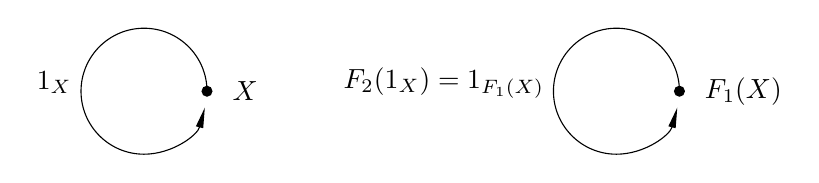
\begin{tikzpicture}[-latex, arrows={-Triangle[angle=20:5pt,scale=1.5]}]
	\fill (0,0) circle (2pt) node [right=2mm] {\(X\)};
	\draw (0,0) arc (0:345: 0.8 cm) node [midway, left] {\(1_X\)};

	\fill (6,0) circle (2pt) node [right=2mm] {\(F_1(X)\)};
	\draw (6,0) arc (0:345: 0.8 cm) node [midway, left] {\(F_2(1_X) = 1_{F_1(X)}\)};
\end{tikzpicture}

\end{document}
